%\clearpage
%\newpage
\section{CONCLUSIONS}
%%\noindent\uline{\textbf{Experiments}}:
%%Writing about cube solid properties\\
%\noindent\uline{\textbf{Discussion}}: 
%\textcolor{blue}{Q2 \& Q3\\
%- Q2: What are the new things you learned after you did whatever you did?\\
%- Q3: What exactly did you do?}
%
%\begin{itemize}
%\color{red}
%\item \textbf{Discussion}
%\item \textit{What your results mean}
%\item \textit{Why it makes a difference}
%\item \textbf{Conclusion}
%\item \textit{Broader implications}
%\item \textit{Areas for further study}
%\end{itemize}
\noindent In this paper, we have proposed a method of closed-path planning for the platonic solids able to successfully generate closed-paths under rolling constraint without sliding. 
%
In particular, the algorithm works by developing the tree exploration method to efficiently search possible paths for cube, tetrahedron, octahedron and icosahedron solids. 
%
In the case of dodecahedron, the initial environments with a gap between two pentagons are vary which may lead to different paths.

 with a gap between two pentagons in the initial environment, the algorithm is be applied to find shortest paths while the other case with overlaps is not guaranteed to find a path.\\


\noindent The results of this study concern path planning in discrete environment through rolling for only platonic solids with free-obstacles.
In future work some more case studies will be included such as rolling platonic solids and the general convex polyhedra with obstacles in the environment. 
Finally, extensions of the proposed algorithm for rolling convex polyhedra on $3D$ convex surface and optimization of the algorithm in storage capacity and executing time will be considered.\\

%\textcolor{blue}{
%\uline{Questions}: Q4. Why should the community care?\\
%\noindent\uline{Should do}: 
%- Overview of Q1, Q2, and Q3; plus\\
%- What does the community still not know?\\
%}
%
%\noindent\uline{Examples}:
%- We have introduced a method of ....\\
%- Most of our effort has focused on .... The results of our method often contain .... We believe that there is significant room for improvement by applying ABC methods to the XYZ problem.\\
%- What do we not do?\\
%
%In this study, we established a method for ... Although we focused on discrete path planning of platonic solid - regular convex polyhedra in known environment, as illustrated using ABC model and EFG example, the developed method/algorithm can be easily implemented to the complex convex polyhedra such as elipsoil ???. The contributions of this study can be summarized as follows:\\
%
%\begin{figure}[h]
%\centering
%	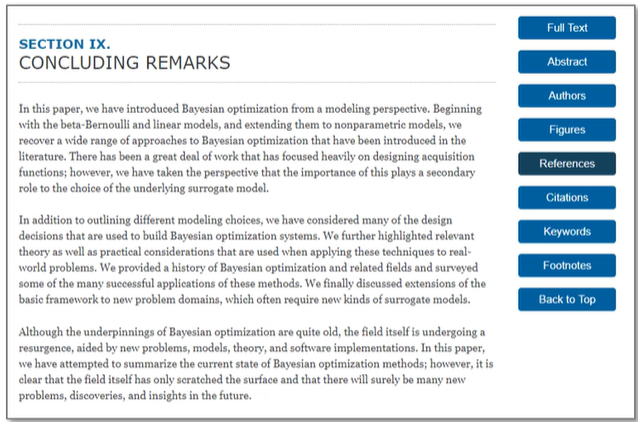
\includegraphics[width=1\textwidth]{image/IEEEDisCon}
%	\caption{First four paths of the cube rolling}
%	\label{fig:Tetra2Case1}
%\end{figure}
